\documentclass[11pt,a4paper]{article}

\usepackage{microtype}
\usepackage{xurl}
\newcommand{\code}[1]{\texttt{\nolinkurl{#1}}}

% Formatting & Input
\usepackage[utf8]{inputenc}
\usepackage[T1]{fontenc}
\usepackage{lmodern}

\usepackage[left=1in,right=1in,top=0.2in,bottom=1in]{geometry}
\usepackage{enumitem}
\setlist{nosep,leftmargin=*}
\setlength{\parskip}{3pt}
\setlength{\parindent}{0pt}

% Math & Figures
\usepackage{amsmath, amssymb}
\usepackage{graphicx}
\usepackage{subcaption}
\usepackage{float}
\graphicspath{{../results/}}
\usepackage{booktabs}
\usepackage{tabularx}
\usepackage{xcolor}

% Hyperlinks
\usepackage{hyperref}
\hypersetup{
    colorlinks=true,
    linkcolor=blue,
    citecolor=blue,
    urlcolor=blue
}

\title{\textbf{Machine Learning Models to Predict Bank Failure within Four Quarters}}
\author{\textbf{AG Team: Greg Pologruto and Andrew Golias}}
\date{}

\begin{document}

\maketitle

\emph{RQ: Can quarterly financial ratios predict failures within four quarters, and do local economic conditions add predictive power beyond the bank's own financials?}

\section{Prediction task and data design}
The analysis uses quarterly bank records from 2007--2012 and 20 predictors covering capital, loan quality, funding, earnings, bank size and charter, plus headquarters-county unemployment and disaster exposure. The training data cover 2007--2010 (13,508 downsampled bank-quarters: 1,228 failures and 12,280 nonfailures); the remaining test set covers 2011--2012 (51,447 bank-quarters, including 320 failures, or 0.622\%). The target is a qualifying failure observed in the following four calendar quarters. A nonfailure requires a complete follow-up window; assistance and mergers are not counted as failures.


To address the rare outcome, training retains all failures and downsamples nonfailures to 9.1\% of the training rows. Predictions are adjusted for the roughly 9.25-to-1 sampling weight before test evaluation:
\[p_{i}=\frac{\hat{y}_i}{\hat{y}_i+(1-\hat{y}_i)\times 9.25}\]
This corrects the probability shift expected from downsampling, assuming the sampled nonfailures represent the larger pool. It preserves the ranking of banks, but probability calibration can still differ across time periods.

\section{Significant Variables}
The strongest signals are bank balance-sheet and credit-quality measures. Total risk-based capital ratio is the leading XGBoost feature by gain. In the data, its median is 6.7\% for failures versus 14.2\% for nonfailures; lower capital therefore marks greater risk. Leverage ratio and equity-to-assets show the same pattern (medians 4.1\% vs. 9.4\%, and 4.4\% vs. 10.0\%). These measures describe the bank’s capital cushion against losses.


Credit stress also separates the groups. Failed banks have a median noncurrent-loan rate of 12.1\%, compared with 1.1\% for nonfailures, and a higher median past-due loans-to-assets ratio. Commercial real estate (CRE) concentration is higher among failures, as is the allowance for loan losses relative to loans. Weaker earnings accompany these risks: median annualized return on assets is -4.7\% for failures and 0.8\% for nonfailures. Together, these patterns are consistent with thinner capital, deteriorating loans, concentrated exposure, and losses preceding failure. They are associations, not causal effects.


\section{Naive Bayes Model}
Naive Bayes is fit on the same training data; its continuous inputs are capped at training-set 1st and 99th percentiles to reduce outlier influence. This model provides a simpler comparison model: it estimates failure risk from each predictor's distribution among failed and surviving banks, then combines those estimates. To limit the effect of extreme values, continuous predictors are capped at their training-set 1st and 99th percentiles. On the test set, it ranks failures nearly as well as XGBoost and identifies 318 of 320 failures in the riskiest 5\% of bank-quarters.


\section{XGBoost Model}
XGBoost is tuned using 2010 as a later-period validation set and refit on 2007--2010. For each bank-quarter, the model estimates whether a qualifying bank failure will be observed in the next four calendar quarters. XGBoost builds shallow decision trees in sequence, with each tree adding a correction to the ensemble's earlier predictions. The sum of tree outputs is the model's raw score, which the binary-logistic objective converts to a failure probability:
\[\hat{y}_i=\sum_{k=1}^{K} f_k(x_i)\]


\section{Test results and interpretation}
Both models are evaluated on the same untouched 2011--2012 set using ROC-AUC, PR-AUC, and the share of failures found when evaluating reporting from bank quarters. They separate failures well in this historical test period: XGBoost ROC-AUC is 0.996 and PR-AUC is 0.558; Naive Bayes scores 0.994 and 0.479. The random-ranking PR-AUC baseline is 0.0062, the test failure rate. When each flags the riskiest 5\% of rows, XGBoost identifies 319 of 320 failures and Naive Bayes 318; precision is about 12.4\% for each. Thus, XGBoost leads on ranking metrics, but their high-recall screening results are very similar.

\begin{figure}[H]
\centering

\begin{subfigure}{0.39\textwidth}
\centering
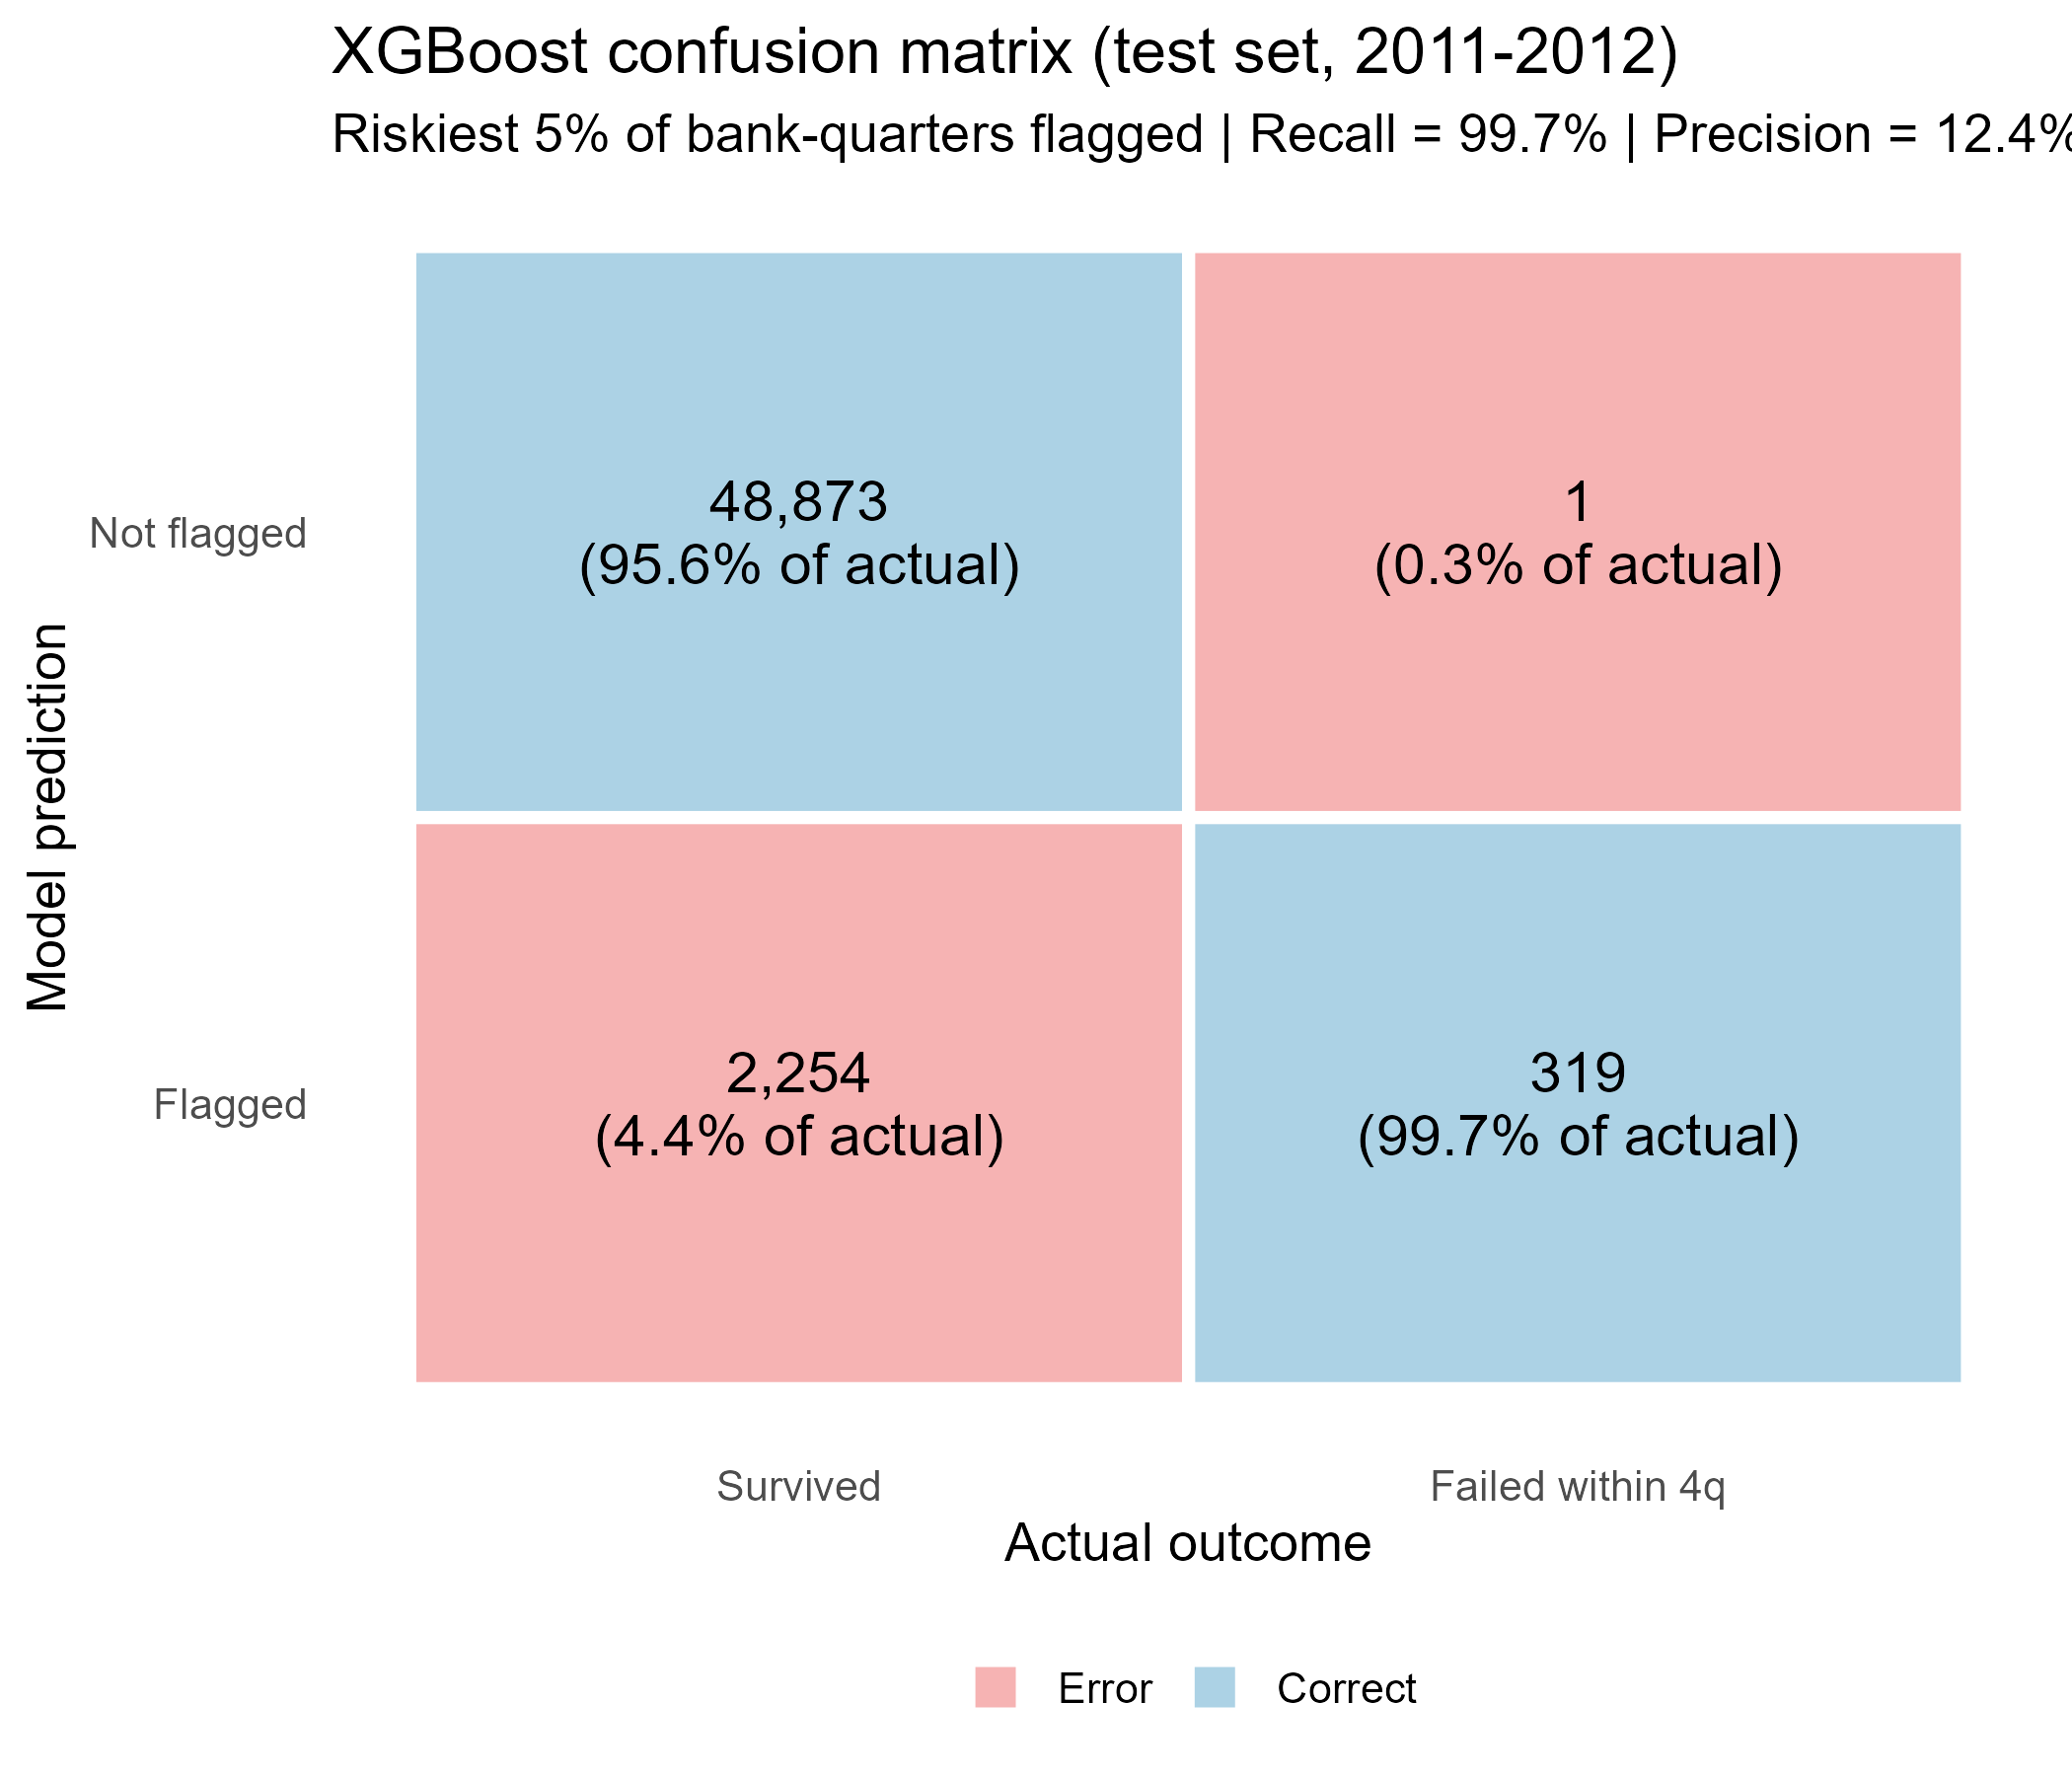
\includegraphics[width=\linewidth,height=0.28\textheight,keepaspectratio]{xgb_confusion_matrix.png}
\caption{XGBoost Confusion Matrix.}
\end{subfigure}
\begin{subfigure}{0.39\textwidth}
\centering
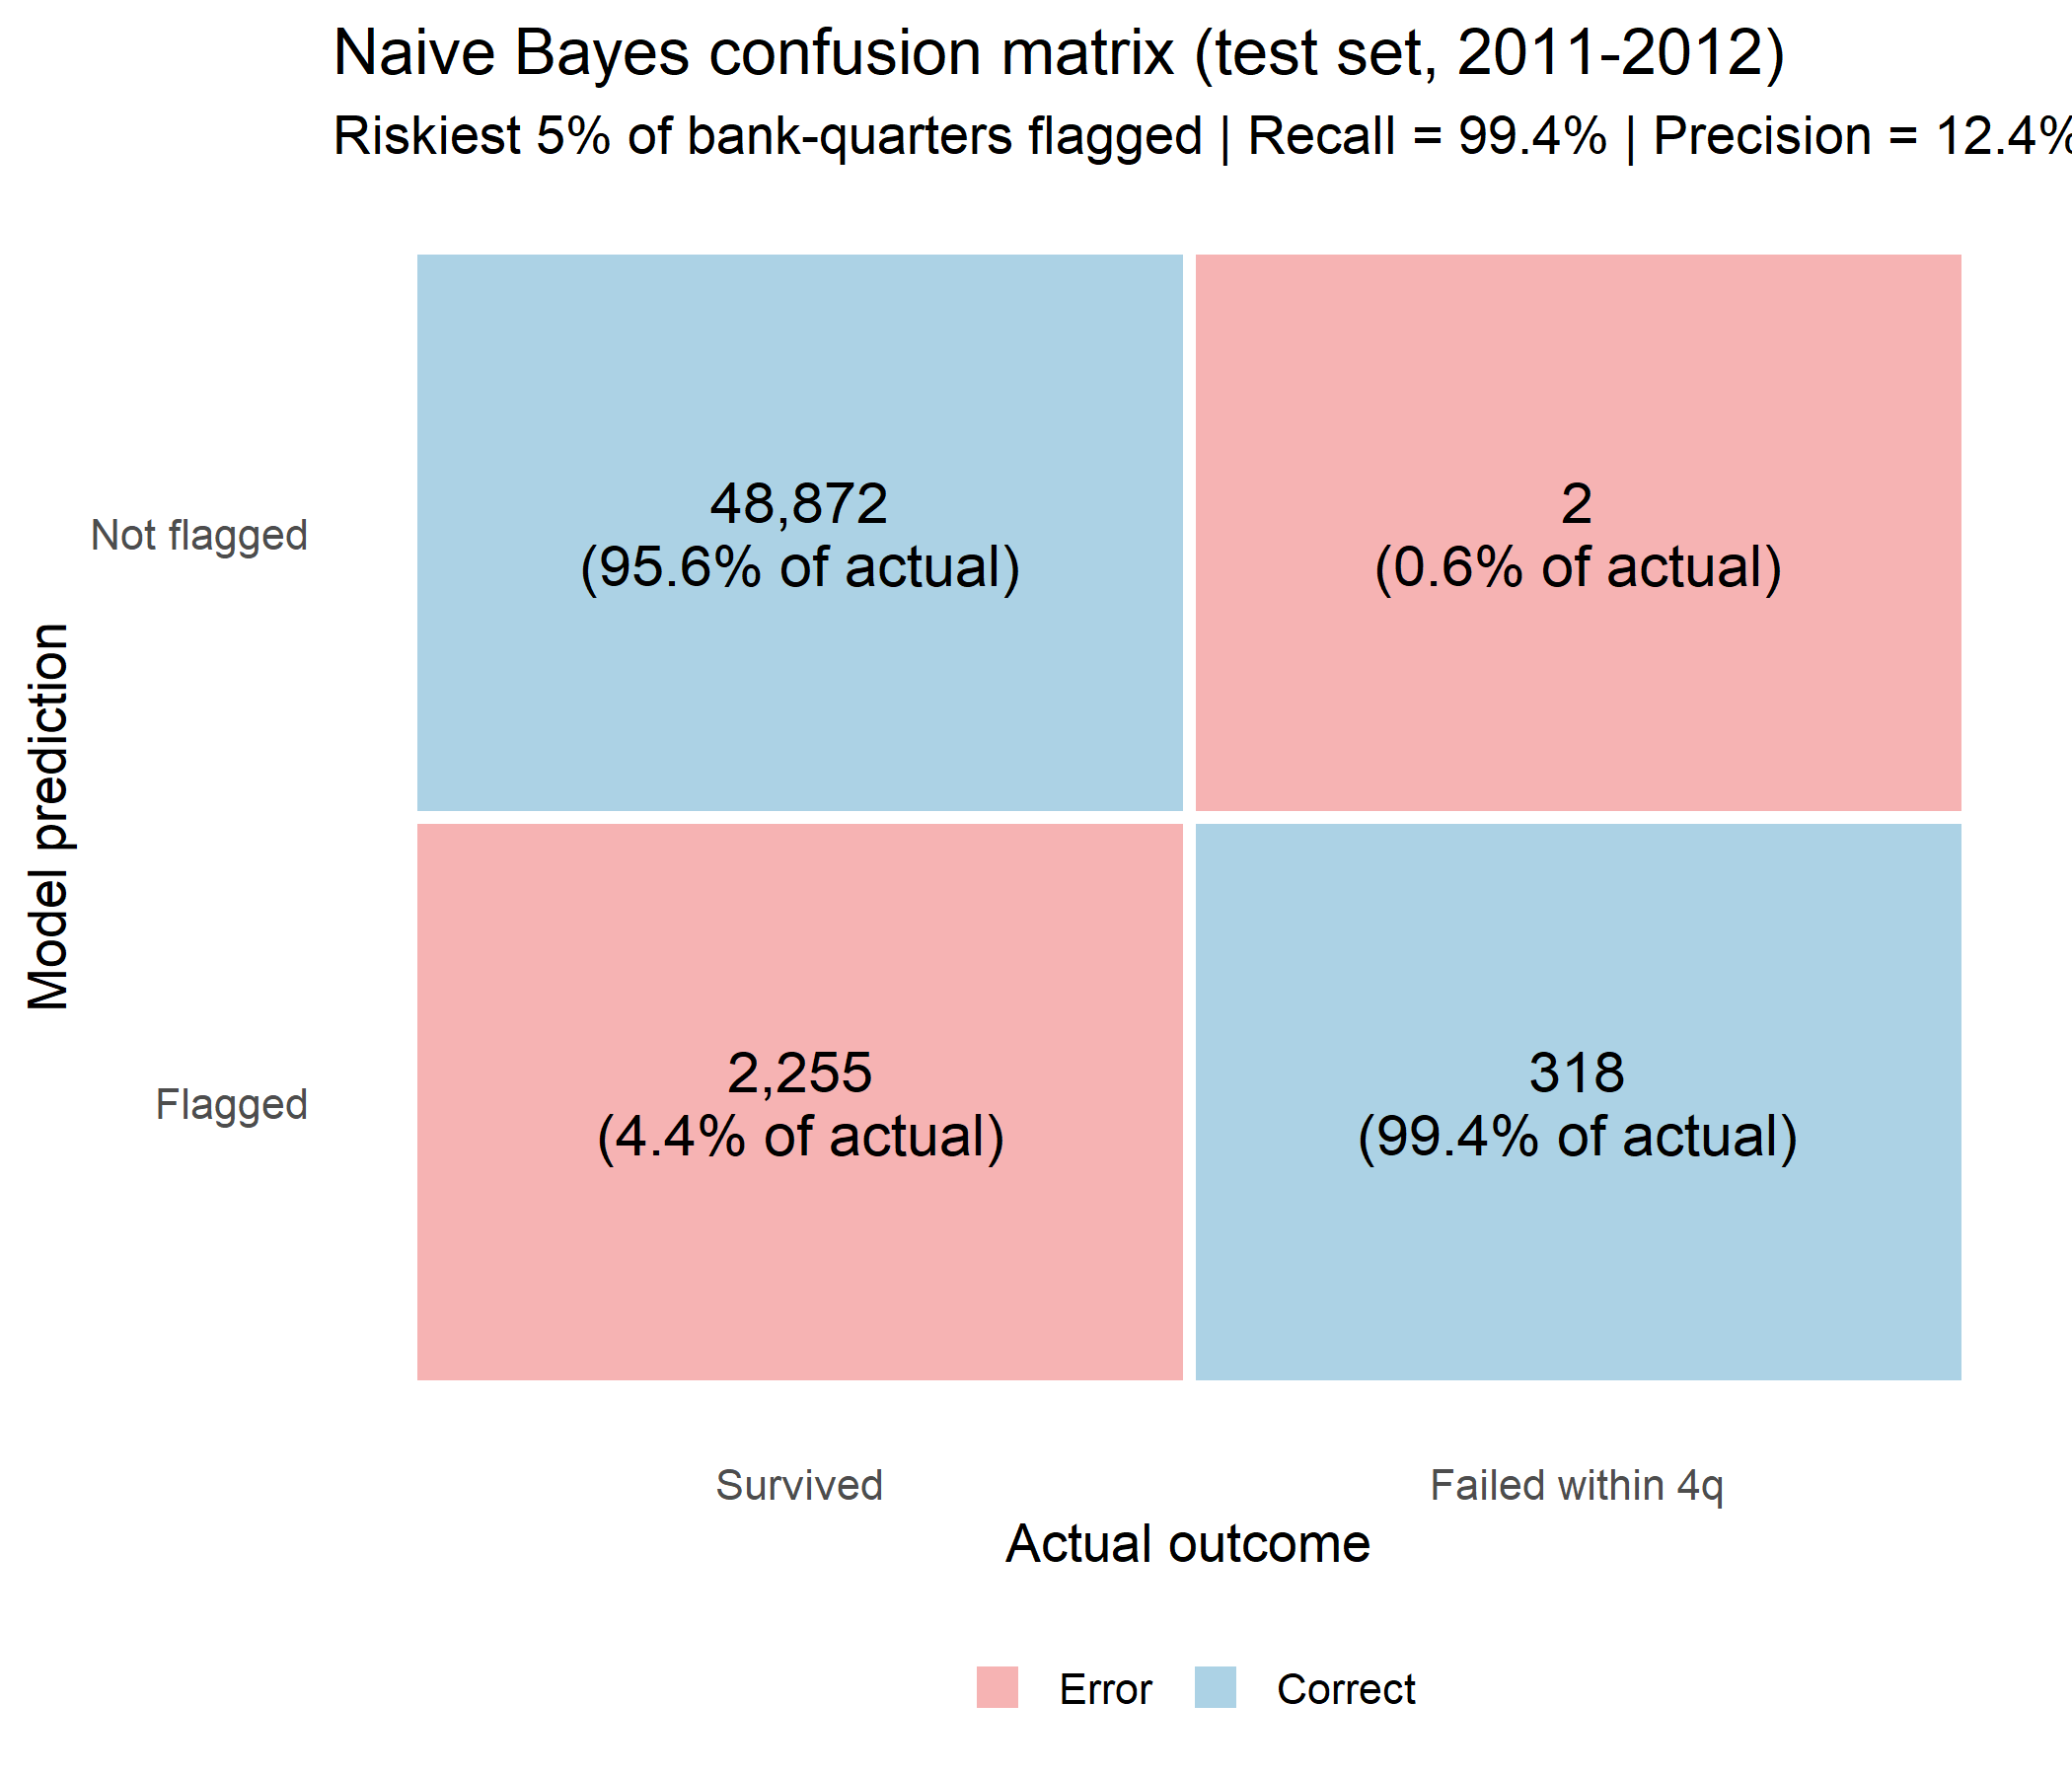
\includegraphics[width=\linewidth,height=0.28\textheight,keepaspectratio]{naive_bayes_confusion_matrix.png}
\caption{Naive Bayes Confusion Matrix.}
\end{subfigure}
\caption{XGBoost vs Naive Bayes model comparison test outcomes.}
\end{figure}


This comparison suggests that model choice alone does not determine useful performance. Both methods benefit from defining the outcome carefully, using a time-based split, limiting extreme values where needed, and making failures visible during training through downsampling. Those data-preparation decisions are central to the strong results; this comparison does not isolate their individual effects, so a controlled evaluation would be needed to measure how much each contributes.


\section{Limitations}
Only a single historical test period is evaluated by either model, so performance does not necessarily carry over to current banks or different economic conditions. Downsampling assumes sampled nonfailures represent the full population; however, probabilities may not hold constant over time. County measures describe headquarters locations and may have a timing delay, impacting the local economic portion of our research.

\end{document}
